%\documentclass[hyperref={pdfpagelabels=false}, aspectratio=43, t, draft]{beamer}  %% Choose aspectratio=43 or aspectratio=169
\documentclass[hyperref={pdfpagelabels=false}, aspectratio=43, t]{beamer}  %% Choose aspectratio=43 or aspectratio=169
%%%%%%%%%%%%%%%%%%%%%%%%%%%%%%%%%%%%%%%%%%%%%%%%%%%%%%%%%%%%%%%%%%%%%%%%%%%%%%%%%%%%%%%%%%%%%%%%%
%%
%%  Die vorliegenden LaTeX-Folien stehen Mitarbeiter*innen und Studierenden der Universität Wien
%%  zur Verfügung und sind ausschließlich zur Verwendung in Forschung und Lehre der Universität  
%%  Wien vorgesehen. Das Copyright der LaTeX-Vorlagen liegt bei der Universität Wien.
%%
%%  These LaTeX slides are available to employees and students of the University of Vienna 
%%  and are intended exclusively for use in research and teaching at the University of Vienna. 
%%  The copyright of the LaTeX templates is held by the University of Vienna.
%%
%%%%%%%%%%%%%%%%%%%%%%%%%%%%%%%%%%%%%%%%%%%%%%%%%%%%%%%%%%%%%%%%%%%%%%%%%%%%%%%%%%%%%%%%%%%%%%%%%



	
%%%%%%%%%%%%%%%%%%%%%%%%%%%%%%%%%
%% ====== Define Style ======= %% 
%%%%%%%%%%%%%%%%%%%%%%%%%%%%%%%%%

%% ======== required inputs ========

	%% ====== title page ======
	\title{Particle Swarm Optimization for Electrical Passivation of Steel Substrate Using Zirconium Oxide} %% Presentation Title
	\newcommand{\titleBackground}{2}    						%% Background graphic: 0 = no; 1 = yes; 2 = yes with more text space
	\newcommand{\gPath}{figures/}									%% set graphics path
	\newcommand{\graphicsTitleBackground}{title}    %% Filename of background graphic


%% ======== optional inputs ========
	
	%% ====== title page ======
	\subtitle{PSO for Steel Passivation with ZrO}  %% (optional) Subtitle, comment out to avoid include
	\newcommand{\authorText}{Johann Dorn}				%% (optional) Author
%	\newcommand{\logoTitleFooterR}{grey}  %% (optional) additional logo in title page footer, most right
%	\newcommand{\logoTitleFooterM}{grey}  %% (optional) additional logo in title page footer, more right (if horizontal spacing not adequate, save multiple logos in one file, use \logoTitleFooterR)
%	\newcommand{\logoTitleFooterL}{grey}  %% (optional) additional logo in title page footer, right (if horizontal spacing not adequate, save multiple logos in one file, use \logoTitleFooterR)

	%% ====== footer ======
	\newcommand{\textFooter}{\subtitle - \authorText} %% (optional) Text for footline, e.g. title, comment out lines to avoid include, max. 1 line
	\newcommand{\slideNumberLabelFooter}{Slide}    	%% Page/Slide/Folie/Seite
	\date{2024-10-30} %% Date, comment out to get current date

	%% ====== header ====== 
	%\newcommand{\sectionHeader}{Section (optional)} %% (optional) Text before section number, e.g. Section or Kapitel; comment out to avoid headline

	%% ====== TOC ====== 
	%\newcommand{\includeTocAtBeginSection}{}   		 %% (optional) Table of contents at begin of every section, comment out to avoid include


%% ======== load beamer style ========
	\usepackage{beamerthemeuniwien2017}
	
	
%%%%%%%%%%%%%%%%%%%%%%%%%%%%%%%%%%%%%
%% ====== Further Preamble ======= %% 
%%%%%%%%%%%%%%%%%%%%%%%%%%%%%%%%%%%%%

%% ====== settings (optional) ======
	\usenavigationsymbolstemplate{}     %% (optional) Comment out to include navigation 

\usepackage{siunitx}
\usepackage{chemformula}
\usepackage{upgreek}
\usepackage{physics}
\usepackage{xcolor}
\newcommand{\red}[1]{\textcolor{red}{#1}}



%%%%%%%%%%%%%%%%%%%%%%%%%%%%%%%%%%%
%% ====== Begin Document ======= %% 
%%%%%%%%%%%%%%%%%%%%%%%%%%%%%%%%%%%

\begin{document}


%% ====== Title Page ======

\maketitle

													
%% ====== Outline at beginning of document ======

%\begin{frame}{Outline (optional)}
%	\tableofcontents							%% (optional) Table of contents, comment out lines to avoid include
%\end{frame}


%% ====== Slides ======
%TODO: - read aqua/good recipe/mars paper
%01. title slide 
	% - aufhänger
	% - AI and PV
	% - Lab or Computer 
%02. agenda
%\begin{frame}{The Iterative Process}
%	\begin{figure}
%		\center
%		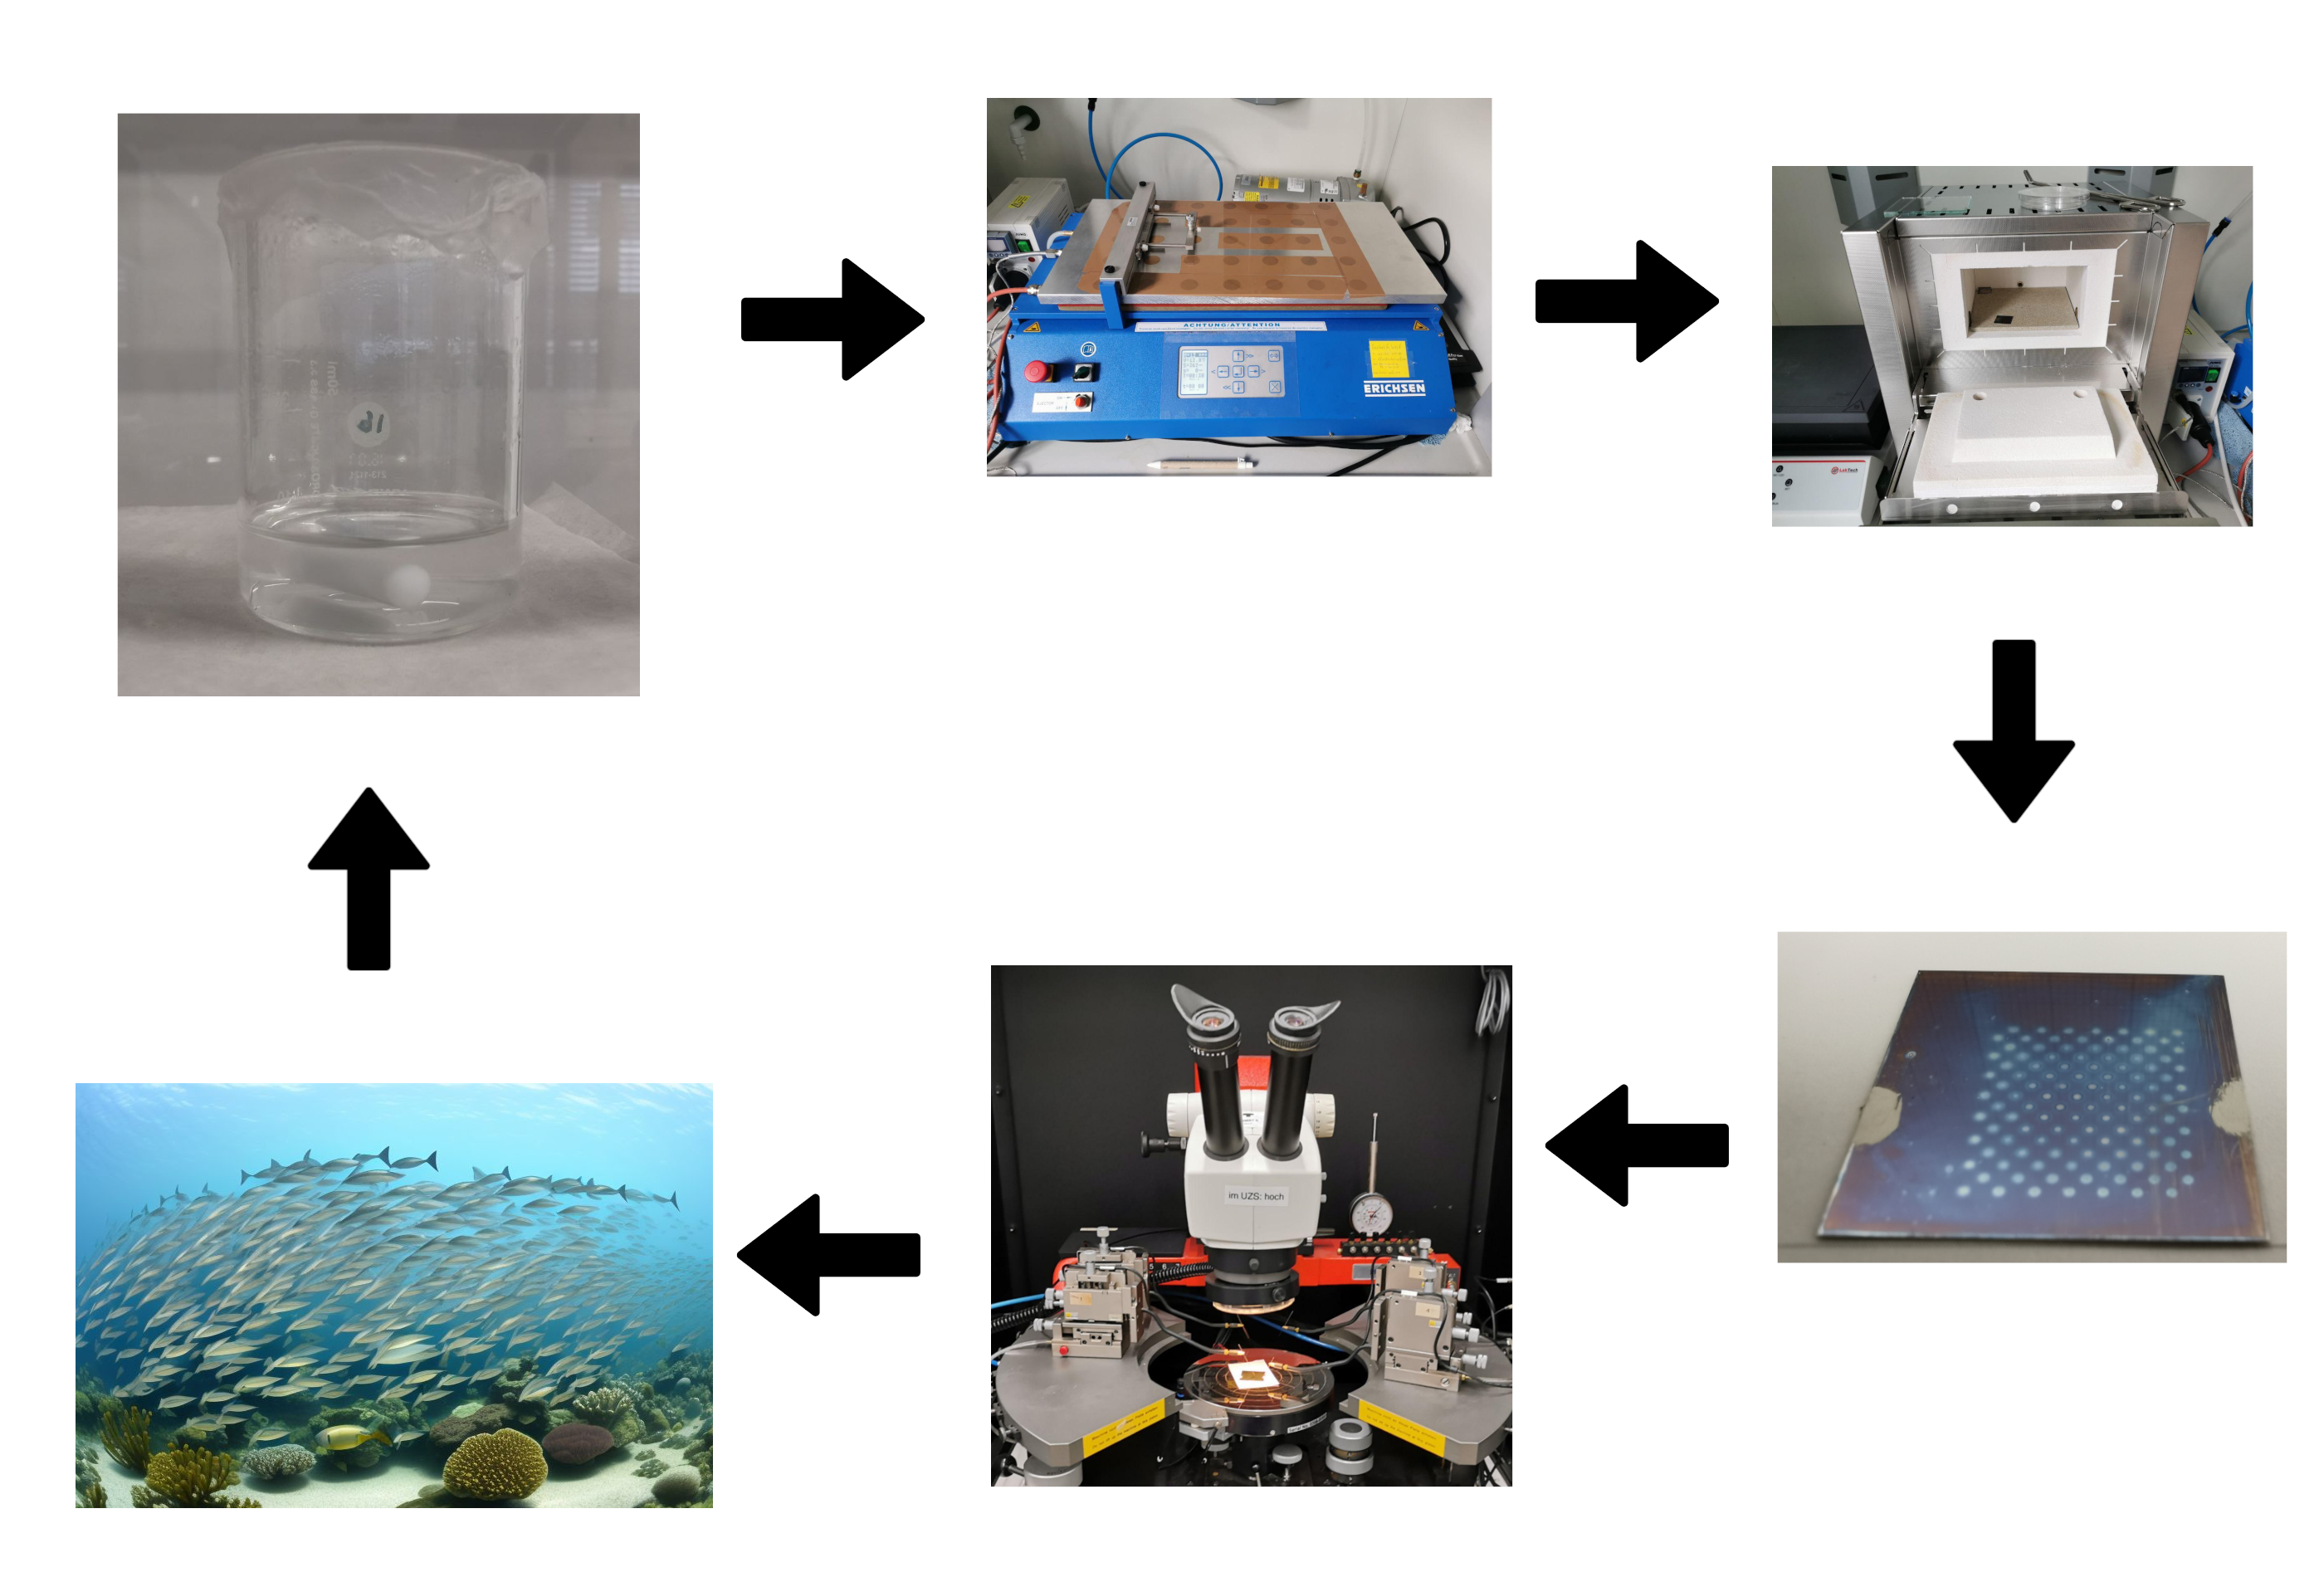
\includegraphics[width=.8\textwidth]{figures/iteration.png}
%	\end{figure}
%\end{frame}
\begin{graphicsFrame}{}{}{0.1}{}{iteration}{}\end{graphicsFrame}
	\iffalse
\begin{frame}{Agenda}
	\vspace{2em}
	\begin{itemize}
		\item Motivation: CIGS substrate
		\item Methods: recipe and sample preparation
		\item Calculation: PSO and data pipeline
		\item Results: materials and optimisation
	\end{itemize}
\end{frame}
\fi
	% - more like process  from beginning to finish
%03. background info
	% - PV CIGS substrate % https://de.wikipedia.org/wiki/Chalkopyrit
	% https://en.wikipedia.org/wiki/Copper_indium_gallium_selenide_solar_cell
\iffalse
\begin{graphicsFrame}{Copper Indium Gallium Selenide (CIGS)}{}{0.37}{left}{cigs}{U. Rau, H.W. Schock (2013) "Solar Cells"}
\begin{table}
	\resizebox{.95\textwidth}{!}{
    \begin{tabular}{cccc}
        \hline\hline
		Empirical Formula&   Band Gap [\SI{}{\electronvolt}]\\
        \hline
		\ch{CuInSe2}&  1.04\\
		\ch{CuGaSe2}&  1.7\\
		\ch{CuInS2}&  1.5\\
		\ch{CuGaS2}&  1.55\\
        \hline\hline
    \end{tabular}
}
    \caption{Band gaps of different chalcopyrites (K. Mertens 2015 "Photovoltaik")}
\end{table}
\end{graphicsFrame}
\fi

\iffalse
\begin{textFrame}{Thin Film Solar Cell}{1}{}
%	\begin{itemize}
%		\item lorem
%		\item ipsum
%		\item \dots
%	\end{itemize}
\begin{table}[tbh]
	\small
    \center
	\resizebox{\textwidth}{!}{
		\begin{tabular}{cccccc}
			\hline
			\hline
			Material&   Type&    Band Gap [\SI{}{\electronvolt}]&    $\lambda$ [\SI{}{\nano\meter}]&    Abs. coef. $\upalpha$ [\SI{}{\centi\meter^{-1}}]    &Penetration Depth [\SI{}{\micro\meter}]\\
			\hline
			c-Si&   indirect&   1.12&   600&    4000&    2.5\\
			c-Si&   indirect&   1.12&   1000&    64&    150\\
			c-Si&   indirect&   1.12&   1100&    3.5&    290\\
			a-Si&   direct&      1.7&    600&    40000&  0.25\\
			CdTe&   direct&      1.45&    600&    37000&  0.3\\
			GaAs&   direct&      1.42&    600&    40000&  0.2\\
			\hline
			\hline
		\end{tabular}
	}
    \caption{Photonic properties of several established PV materials (K. Mertens 2015 "Photovoltaik")}
	\label{tab:cigs:alpha}
\end{table}
\end{textFrame}
\fi

%\begin{graphicsFrame}{Thin-Film Photovoltaics: CIGS modules}{}{0.1}{}{cigs_mod}{}
	\begin{frame}{Thin-Film Photovoltaics: CIGS modules}
	\begin{itemize}
		\item high absorption coefficient
		\item connected in series 
		\item substrate:
			\begin{itemize}
				\item must be insulating 
				\item mostly glass
			\end{itemize}
	\end{itemize}
	\begin{figure}
		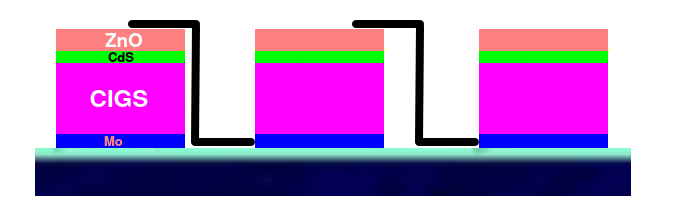
\includegraphics[width=.9\textwidth]{figures/cigs_mod.png}
	\end{figure}
\end{frame}
%\end{graphicsFrame}

%04. hypothesis 
%05. manual methods
	% - precursor solution preparation 
		% Anwar 2017 https://iopscience.iop.org/article/10.1088/1757-899X/257/1/012087
		% Hu 2016 https://www.sciencedirect.com/science/article/abs/pii/S0272884216312548
\begin{frame}{Adaption of Precursor Solutions Recipe}
	\begin{figure}
		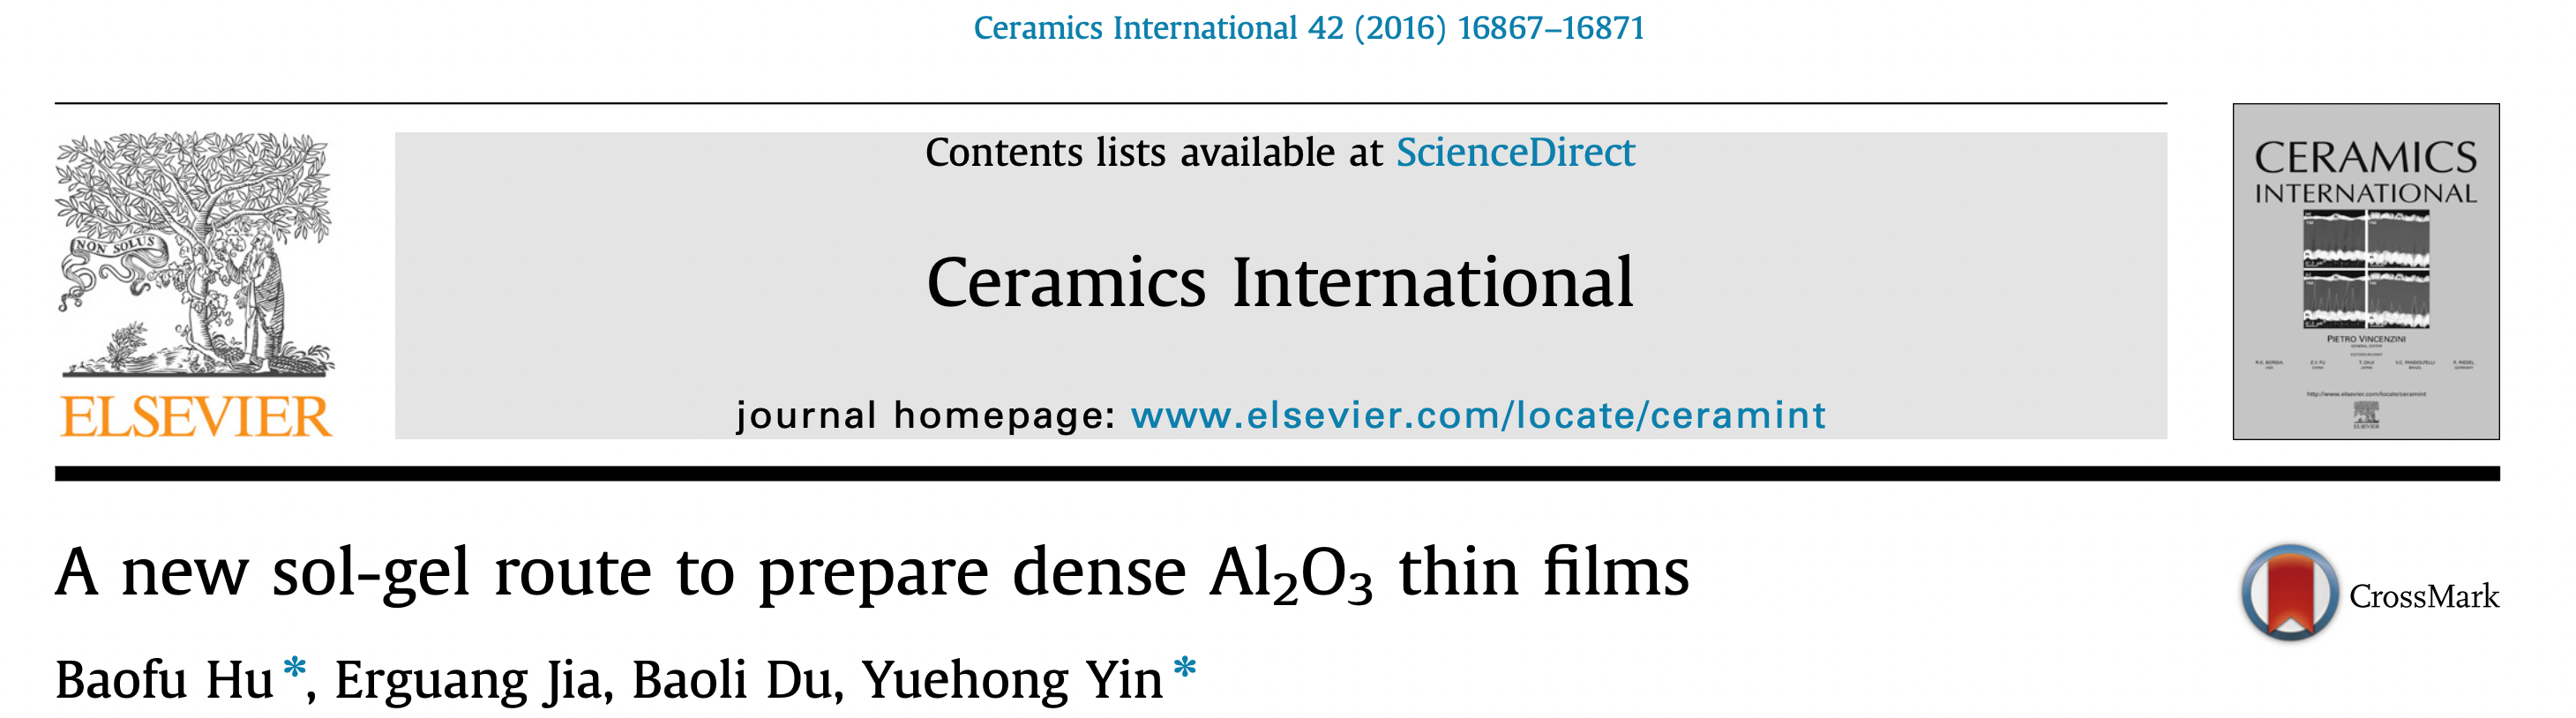
\includegraphics[width=.79\textwidth]{figures/huetal.png}
	\end{figure}
	\pause
\begin{table}[h]
	\center
	\begin{tabular}{lll}
		\hline\hline
		recipe	&original	&adapted \\
		\hline
		solvent & \ch{EtOEt} & \ch{BuOH} \\
		precusor & \ch{Al(OPr^i)3} & \ch{Zr(OPr)4} \\
		chelating agent & \ch{AcAc} & \ch{AcAc} \\
		stabilzing agent & \ch{AcOH} & \ch{iPrOH}/\ch{AcOH}	\\
		\hline\hline
	\end{tabular}
	%\caption{Composition of different buthanolic solutions}
\end{table}
\end{frame}
%\iffalse
\begin{frame}{Different Precusor Concentrations}
	\begin{figure}
		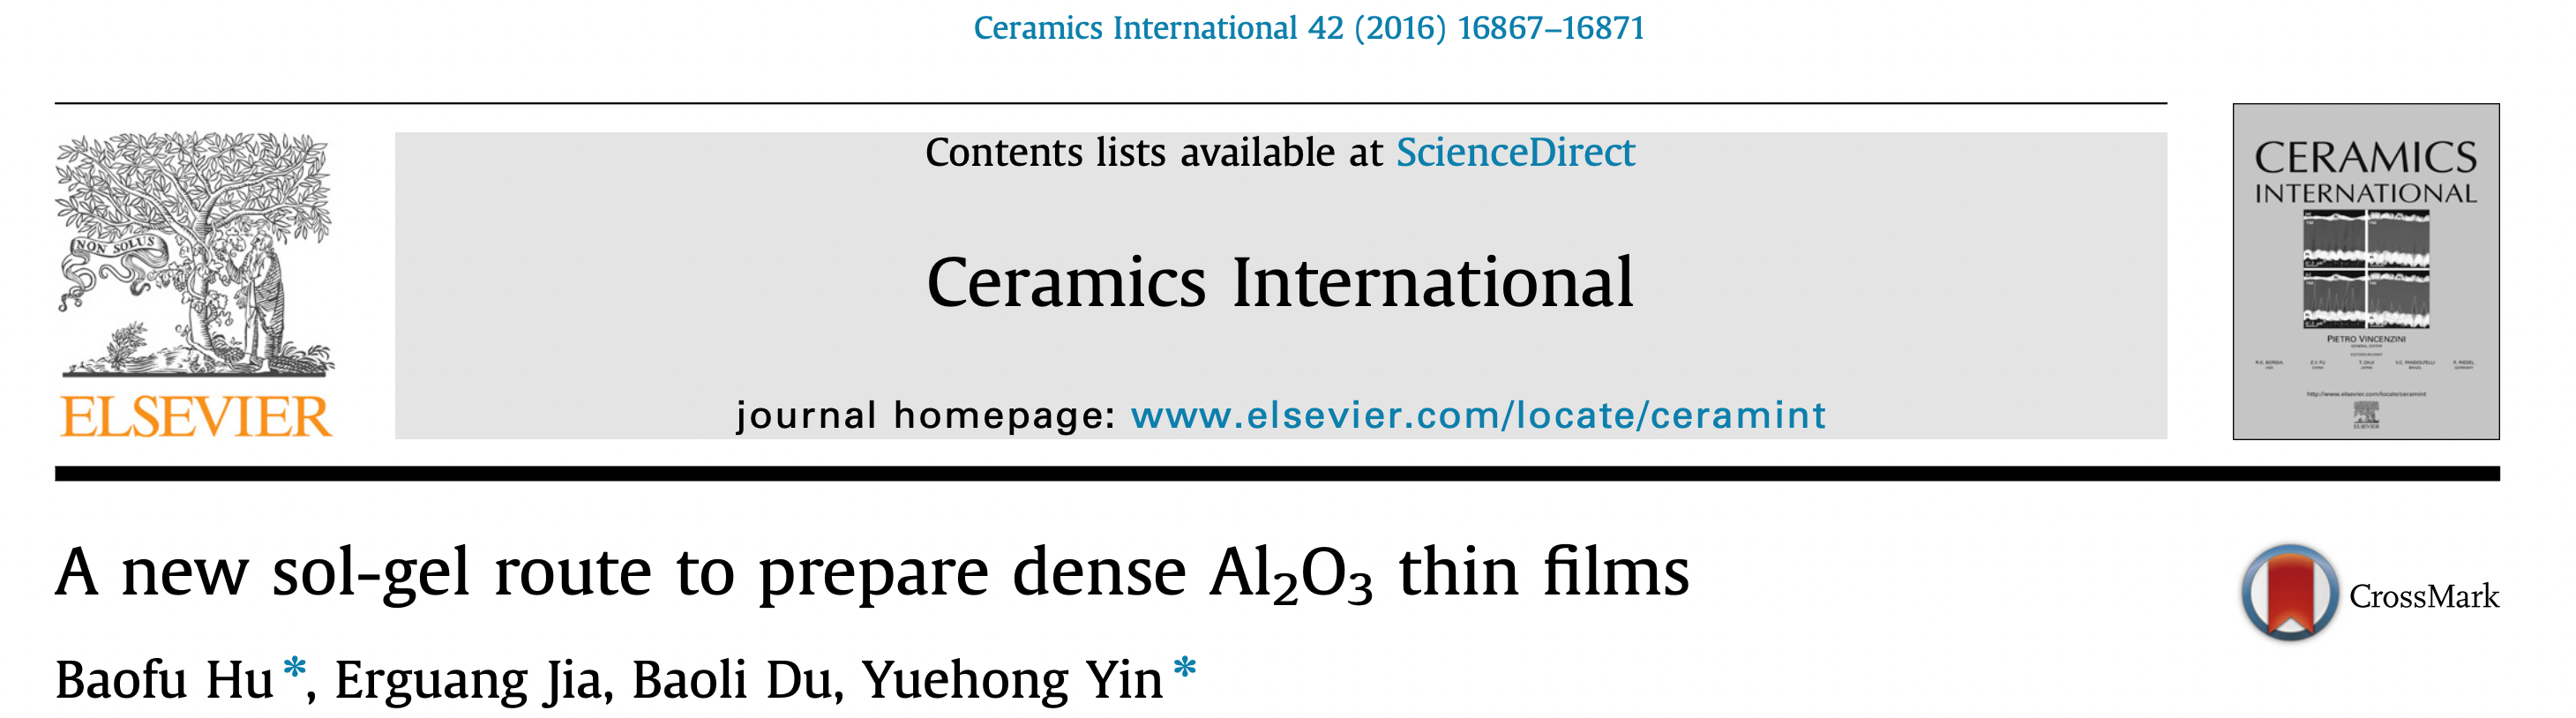
\includegraphics[width=.79\textwidth]{figures/huetal.png}
	\end{figure}
\begin{table}[h]
	\center
	\label{tab:rec2}
	\begin{tabular}{rlllll}
		\hline\hline
		&\red{1x}		&2x		&3x		&4x		&5x		\\
		\hline
		\ch{BuOH} [ml]	&\red{4.95}	&4.9	&4.85	&4.8	&4.75	\\
		\ch{ZrPro} [ml]	&\red{0.05}	&0.1	&0.15	&0.2	&0.25	\\
		\ch{AcAc} [ml]	&\red{0.0125}	&0.025	&0.0375	&0.05	&0.0625	\\
		\ch{IPO}/\ch{AcOH} [ml]	&\red{2}		&2		&2		&2		&2		\\
		\hline\hline
	\end{tabular}
	%\caption{Composition of different buthanolic solutions}
\end{table}
%\fi
\end{frame}

	% - doctor blading = tape castig 
	% - calcination 
\begin{graphicsFrame}{Tape Casting and Calcination}{}{0.37}{left}{tc}{}

		\vspace{1em}
		\begin{itemize}
			\item Tape Casting
				\begin{itemize}
					\item temperature: 40-80\SI{}{\degreeCelsius}
					\item blade speed: 10-20\SI{}{\milli\meter/\second}
				\end{itemize}
				\vspace{1em}
			\item Calcination
				\begin{itemize}
					\item temperature: 300-500\SI{}{\degreeCelsius}
					\item heating rate: 2-18\SI{}{\degreeCelsius/\minute}
				\end{itemize}
		\end{itemize}
\end{graphicsFrame}

	% - SEM % check which sample 
\begin{graphicsFrame}{Cross Section of \ch{ZrO2}}{}{0.37}{right}{sem_cs}{}
	\vspace{3em}
		\begin{itemize}
			\item Scanning Electron Microscope 
			\item substrate: FTO (Fluorine Doped Tin Oxide)
			\item single layer of \ch{ZrO2}
		\end{itemize}
\end{graphicsFrame}

%\begin{frame}{Tape casting and Calcination}
%	\begin{figure}
%		\center
%		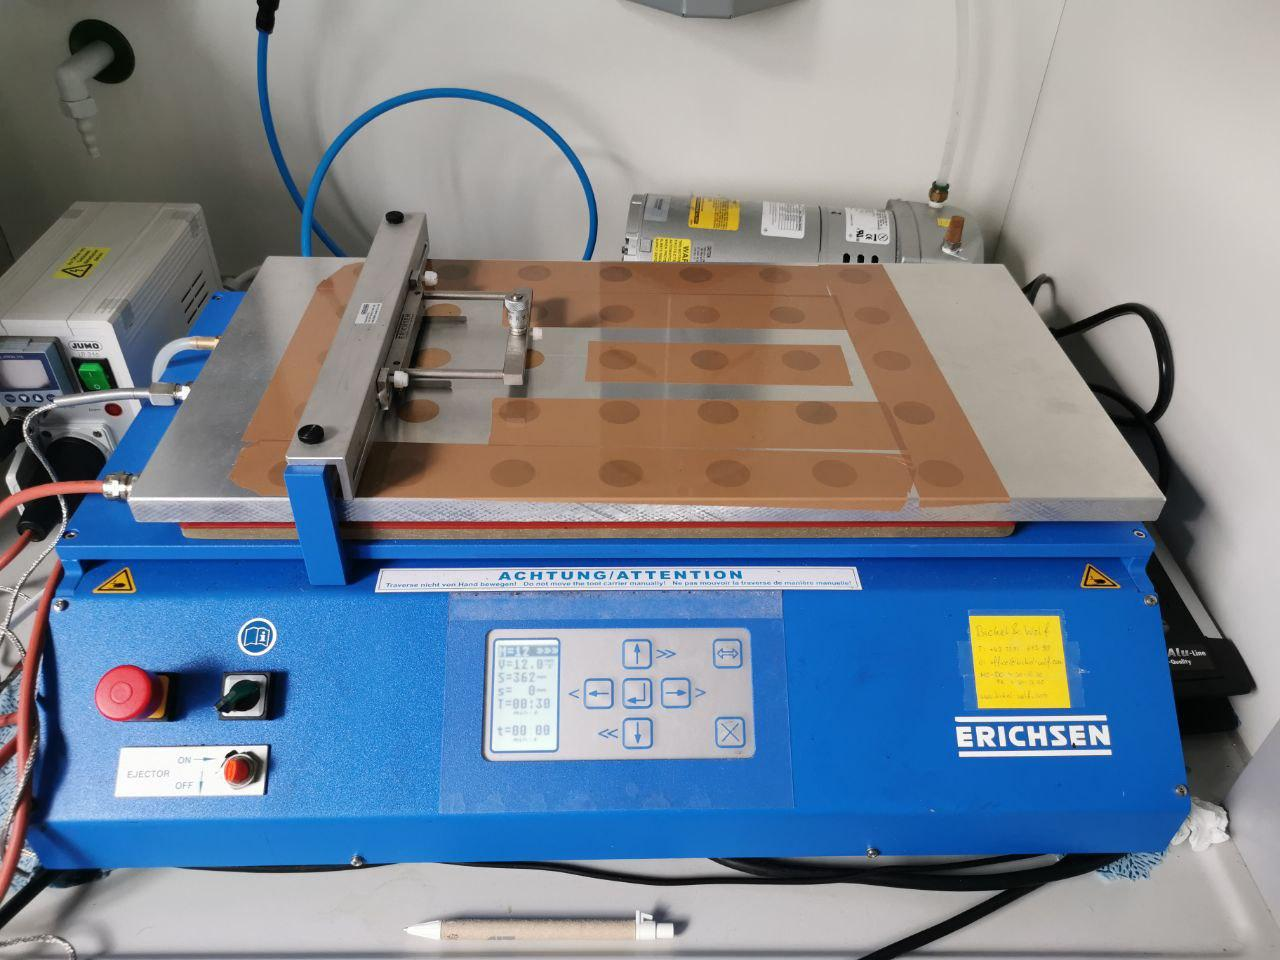
\includegraphics[width=.65\textwidth]{figures/tc.jpg}
%	\end{figure}
%\end{frame}
%	\begin{itemize}
%		\item doctor blading construction 
%		\item calcination infos (max temperatur, heating rate)
%	\end{itemize}
%\end{frame}
	% - sputtering contacts
	% - measuring current-voltage characteristics
\iffalse
\begin{frame}{Application of Contacts}
	\begin{figure}
		\includegraphics<1>[width=.63\textwidth]{figures/sample1.jpg}
		\includegraphics<2>[width=.63\textwidth]{figures/sample2.jpg}
		\includegraphics<3>[width=.63\textwidth]{figures/sample3.jpg}
	\end{figure}
\end{frame}
\fi
%\begin{graphicsFrame}{Application of Contacts}{}{0.37}{right}{sample1}{}
%		\begin{itemize}
%			\item Left: Shadow mask
%			\item Right: Steel substrate \ch{ZrO2} layer
%		\end{itemize}
%\end{graphicsFrame}
%
\begin{graphicsFrame}{Application of Contacts}{}{0.37}{left}{sput1}{}
		\begin{itemize}
			\item Bottom left: Shadow mask
			\item Bottom right: Steel substrate \ch{ZrO2} layer
			\item Top: samples with mask attached
		\end{itemize}
\end{graphicsFrame}
%
\begin{graphicsFrame}{Applied Contacts}{}{0.37}{right}{sample2}{}
	\vspace{1em}
		\begin{itemize}
			\item passivated sample with array of contacts
				\vspace{.5em}
			\item contacts to steel on edges
		\end{itemize}
\end{graphicsFrame}
%
\begin{graphicsFrame}{Measuring Current Voltage Characteristics}{}{0.37}{left}{sample3}{}
	\vspace{3em}
		\begin{itemize}
			\item left needle touches top contact (\ch{ZrO2})
				\vspace{1.5em}
			\item right needle touches bottom contact (steel)
		\end{itemize}
\end{graphicsFrame}

	% - I-V % https://en.wikipedia.org/wiki/Current%E2%80%93voltage_characteristic
\begin{graphicsFrame}{Current-Voltage characteristics}{}{0.37}{left}{iv-noi}{}
	\vspace{2em}
	\begin{itemize}
		\item voltage sweep
		\vspace{.5em}
		\item 10\SI{}{\milli\volt} steps
		\vspace{.5em}
		\item very low current 
		\vspace{.5em}
		\item low conductivity 
		\vspace{.5em}
		\item high resistance 
	\end{itemize}
\end{graphicsFrame}
\begin{graphicsFrame}{Current-Voltage characteristics II}{}{0.37}{left}{iv-log}{}
	\vspace{2em}
	\begin{itemize}
		\item all measurements of single sample
		\vspace{.5em}
		\item huge range 
		\vspace{.5em}
		\item low current
		\vspace{.5em}
		\item high current
	\end{itemize}
\end{graphicsFrame}

%06. computational pipeline 
\begin{graphicsFrame}
	{Pin Hole Density and Leakage Current}
	{}{0.37}
	{left}{calc}{}
	\vspace{2em}
	\begin{itemize}
		\item Conductivity
			\begin{itemize}
				\item $
					g = \eval{\dv{I}{V}}_{V =0}
					$
			\end{itemize}
	\vspace{0.5em}
%	\pause
		\item Pin Hole Density 
			\begin{itemize}
				\item $
	s_i = \begin{cases}
		1 &\text{if} \quad g_i < 10^{-5} \\
		0 &\text{if} \quad g_i \geq 10^{-5} \\
%        1 &\text{if} \quad -log_{10}(g_i) < 5 \\
%        0 &\text{if} \quad -log_{10}(g_i) \geq 5 \\
	\end{cases}
					$
				\item $
	\rho = \sum_i^N \frac{s_i}{N}
					$
			\end{itemize}
	\vspace{0.5em}
%	\pause
		\item Leakage Current 
			\begin{itemize}
				\item $
    \gamma = \sum_i^N \frac{ (-log_{10}(g_i) - 13)^2}{N}
	$
			\end{itemize}
	\end{itemize}
\end{graphicsFrame}
	% - PSO + MARS = EMMA
	% PSO https://doi.org/10.1109/CEC.2010.5586165
\begin{graphicsFrame}{Particle Swarm Optimisation}{}{0.37}{right}{swarm}{}
	\vspace{3em}
	\begin{itemize}
		\item inspired by fish schools %# swarm intelligence
		\item iterative process % nice bcs sample prep takes long time 
		\item particles: 
			\begin{itemize}
				\item input vars: position 
				\item velocity
			\end{itemize}
		\item next times step
		\item R package \texttt{emma} 
	\end{itemize}
\end{graphicsFrame}

\begin{frame}{Input Variables for Optimisation}
	\begin{itemize}
		\item precursor solution concentration
		\item number of layers 
		\item coating temperature
		\item blade speed
		\item calcination temperature
		\item calcination heating rate
	\end{itemize}
\end{frame}

\begin{frame}{Input Variables for Optimisation}
\begin{table}[htb]
	\centering
	\begin{tabular}{cc cc cc}
		\hline\hline
		$c_{zr}$ [22\SI{}{\milli\mol/\liter}]	&$n_L$	&$T_{C}$[\SI{}{\degreeCelsius}]	&$v_{C}$[\SI{}{\milli\meter/\second}]	&$T_{cal}$[\SI{}{\degreeCelsius}]	&$v_{cal}$[\SI{}{\degreeCelsius/\minute}]	\\
		\hline
%		\pause
		2				&4		&40					&10				&300				&2	\\
		3				&6		&50					&12				&400				&6	\\
		4				&8		&60					&14				&500				&10	\\
		5				&10		&70					&16				&					&14	\\
						&12		&80					&18				&					&18	\\
						&		&					&20				&					& \\
		\hline\hline
	\end{tabular}
	\caption{Discrete levels of each input parameter }
	\label{tab:input}
\end{table}
\end{frame}

%	\begin{itemize}
%		\item Aluminium Contact through mask
%		\item Silver paste
%	\end{itemize}
%\end{frame}
%07. results measuring 
%\begin{graphicsFrame}{I-V characteristics}{}{0.1}{}{iv2}{}\end{graphicsFrame}
%\begin{graphicsFrame}{I-V characteristics}{}{0.1}{}{iv3}{}\end{graphicsFrame}
	% - EMMA 
%08. results EMMA 
%\begin{frame}{Pin Hole Density}\begin{figure}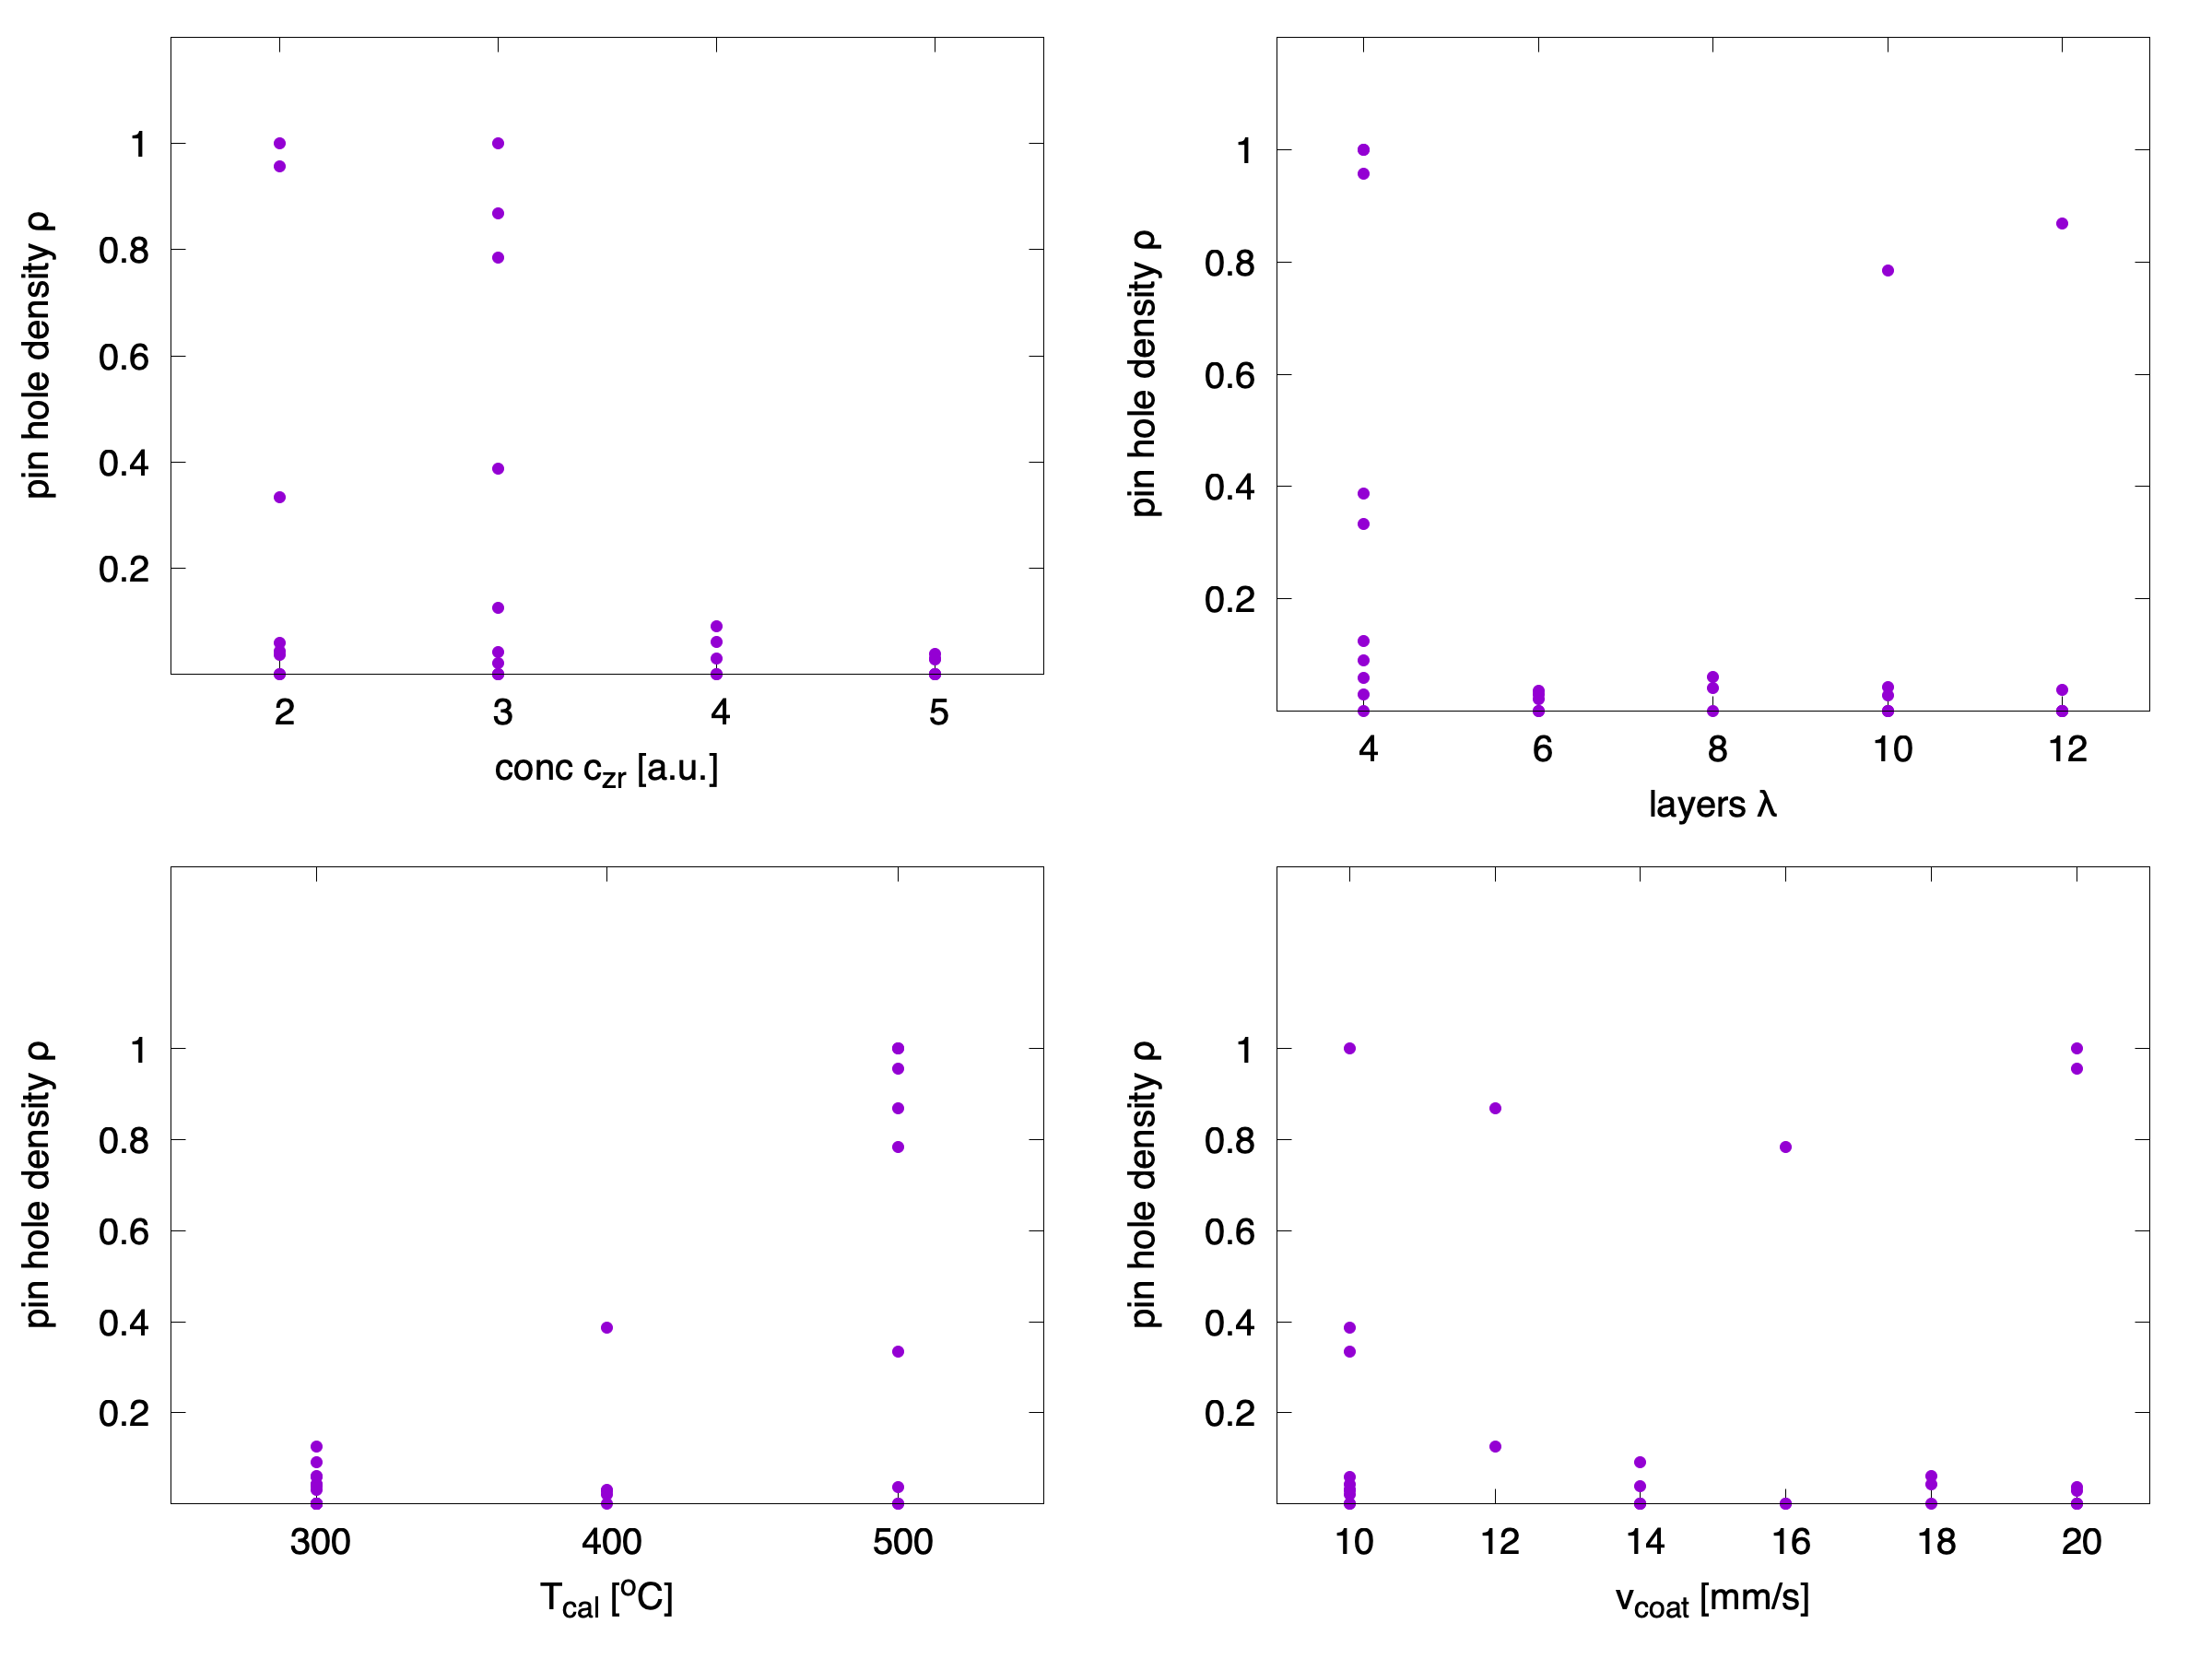
\includegraphics[width=.66\textwidth]{figures/phd.png}\end{figure}\end{frame}
%\begin{frame}{Leakage Current}\begin{figure}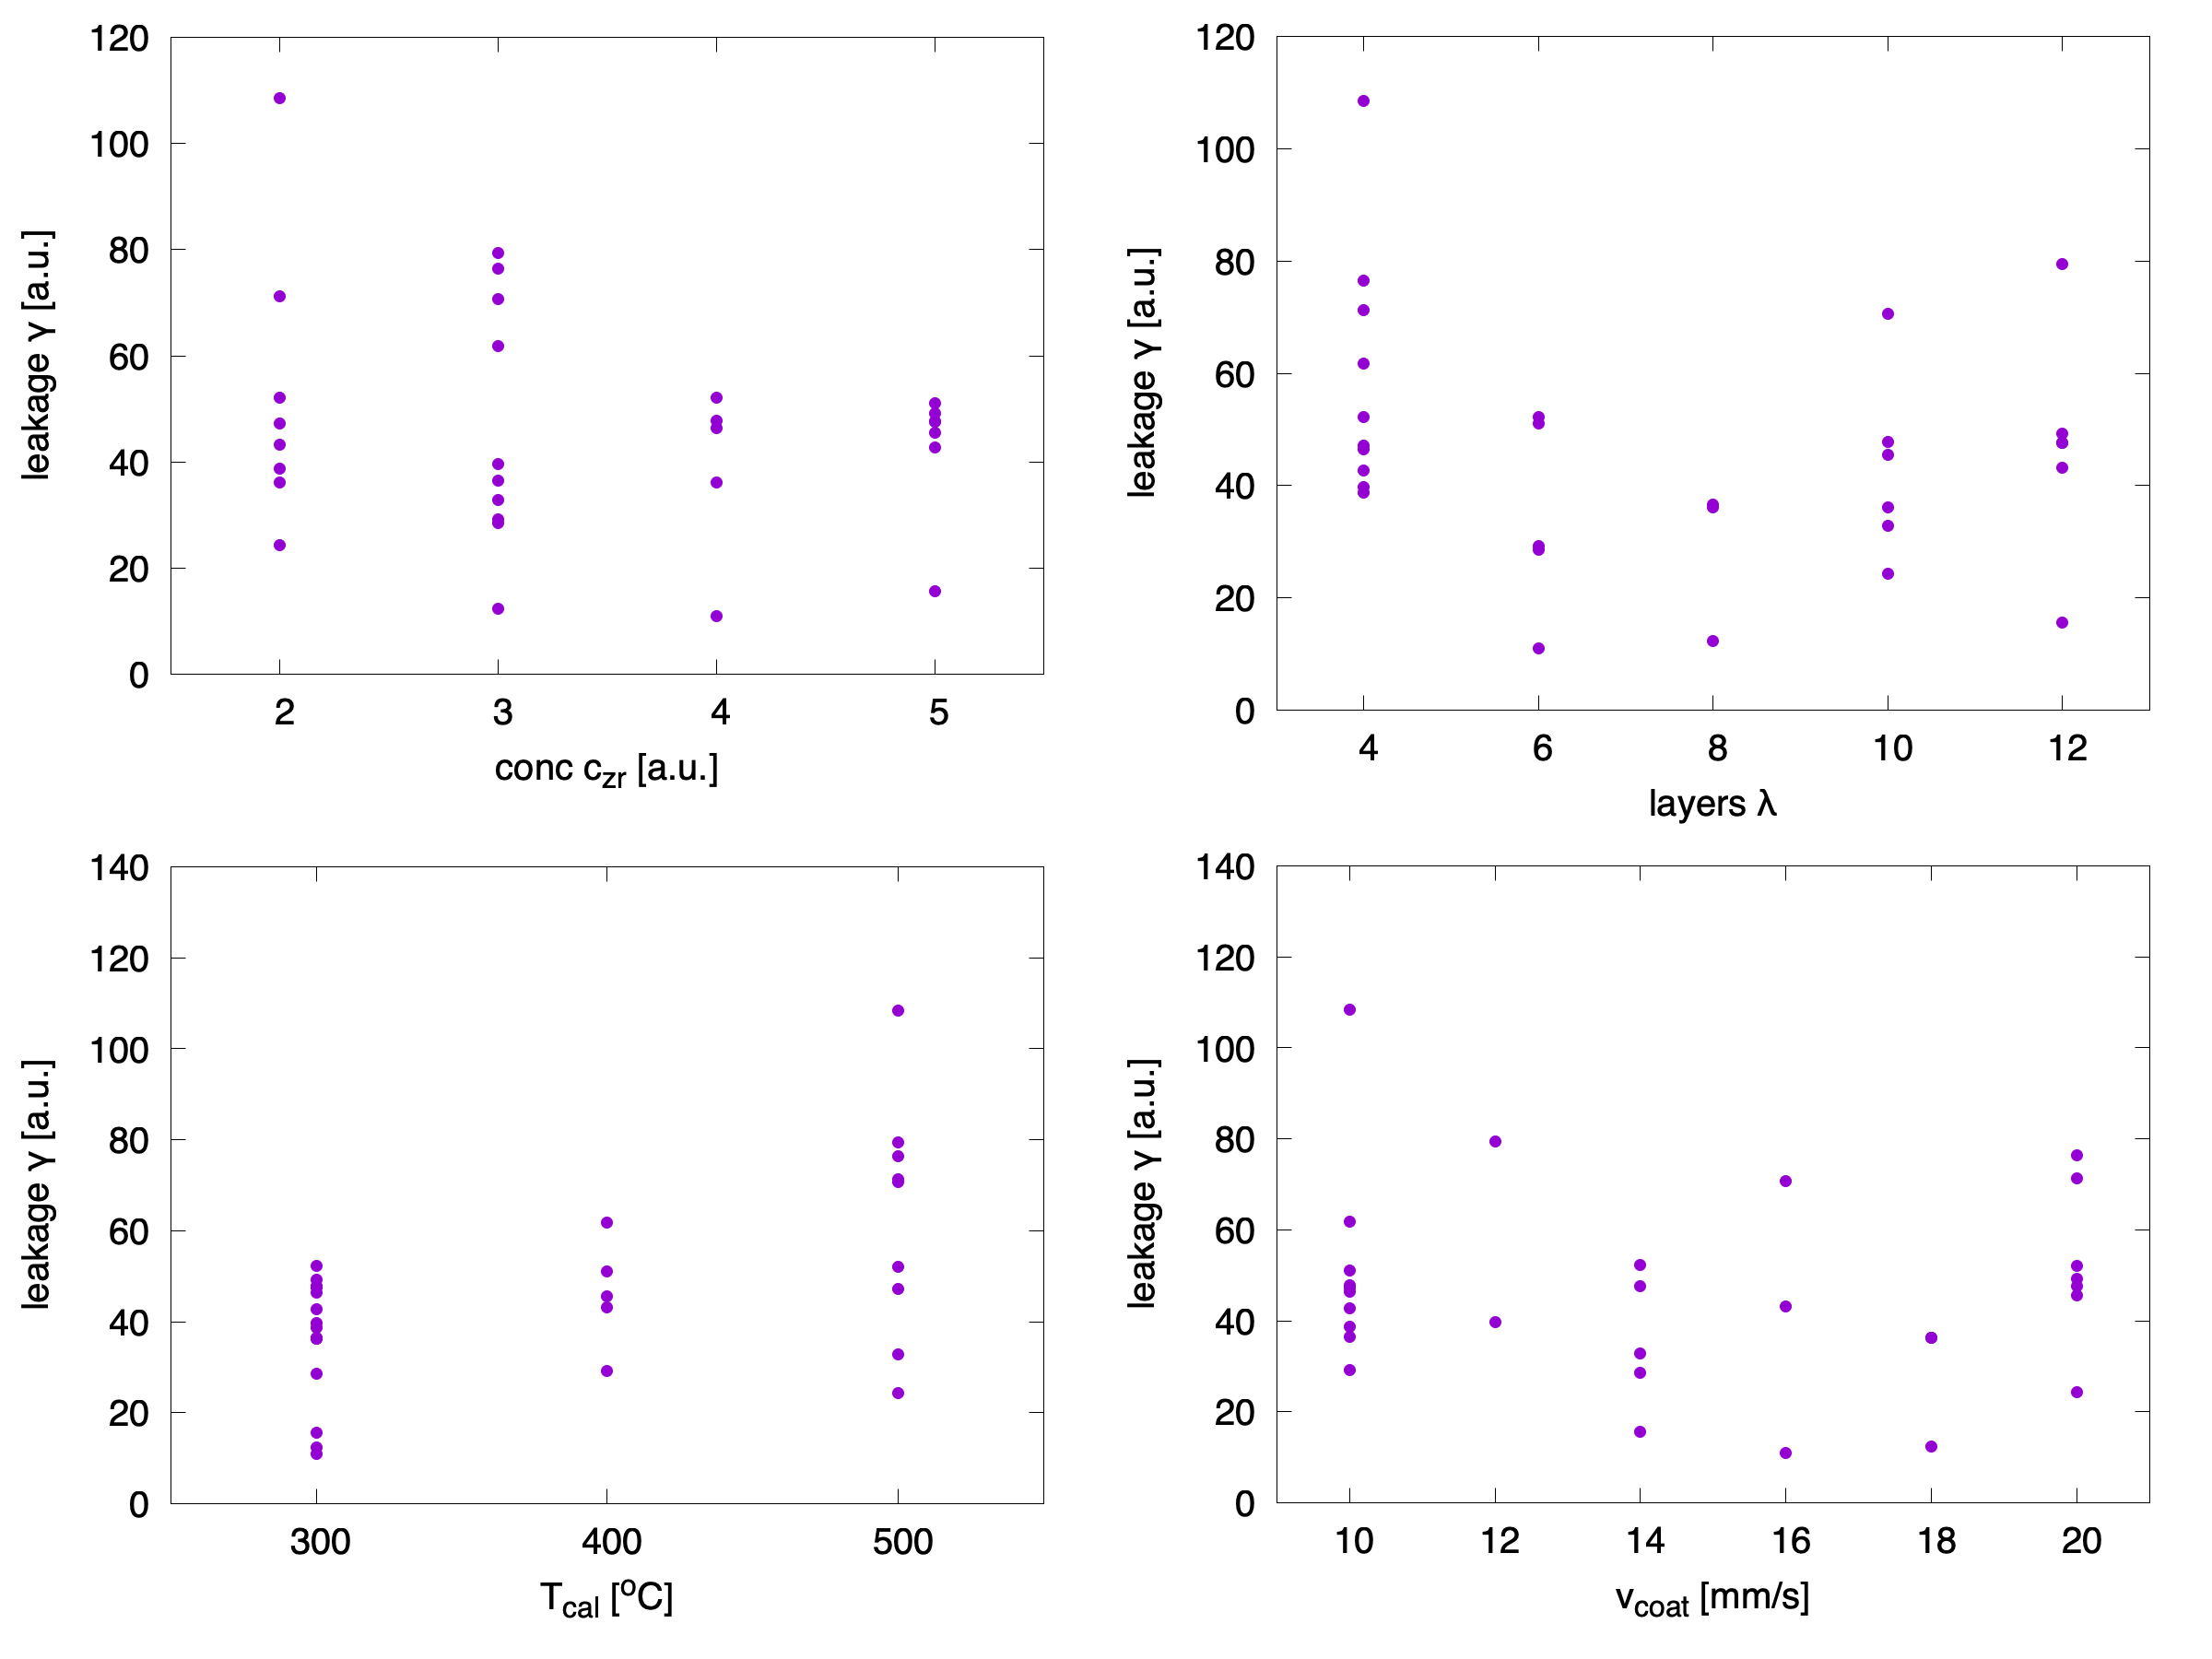
\includegraphics[width=.66\textwidth]{figures/leakage.png}\end{figure}\end{frame}
\begin{frame}{Particle Swarm Optimisation Iterations}
	\begin{itemize}
		\item metrics are reduced per generation
		\item model learned to represent data
	\end{itemize}
	\begin{figure}
		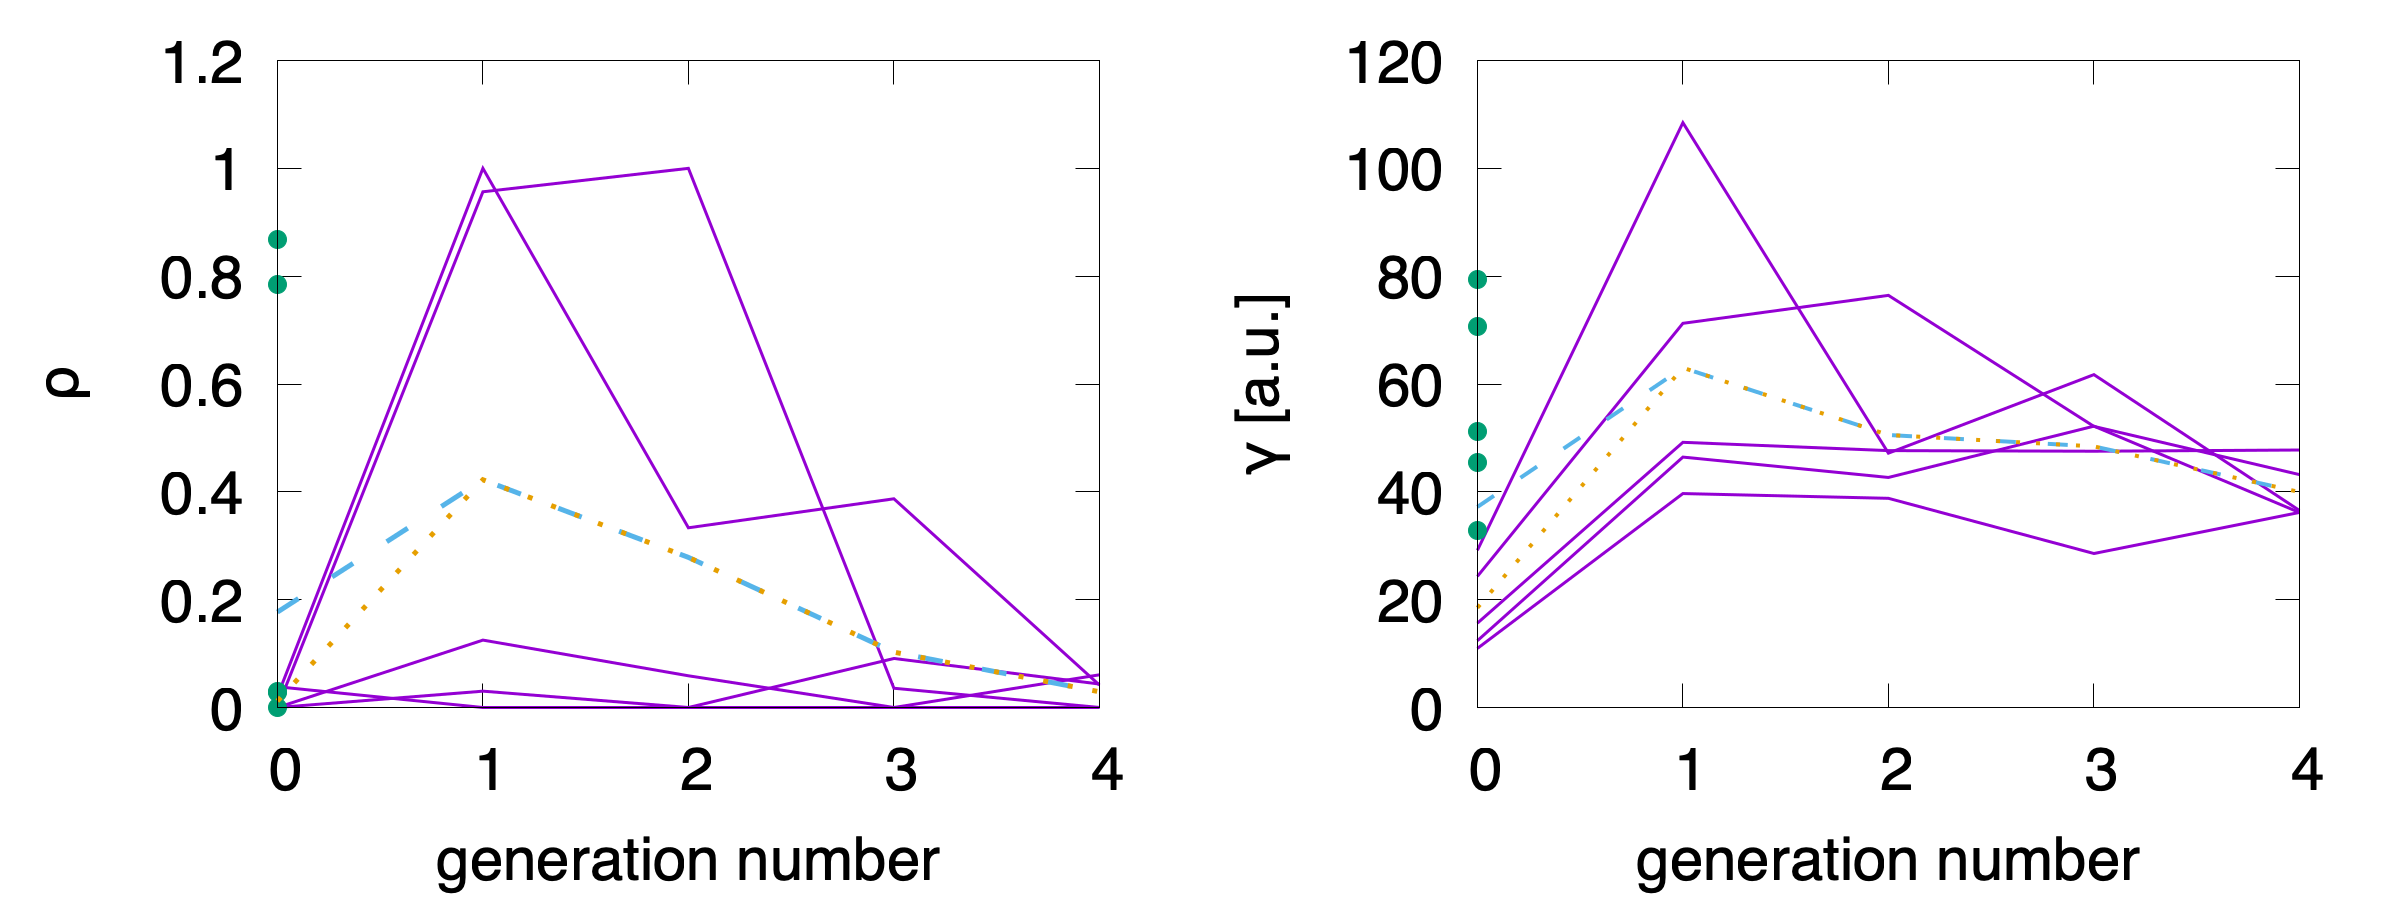
\includegraphics[width=.96\textwidth]{figures/emma-gen.png}
	\end{figure}
\end{frame}

%\begin{graphicsFrame}{Pin Hole Density}{}{0.1}{}{phd}{}\end{graphicsFrame}
%\begin{graphicsFrame}{Pin Hole Density}{}{0.1}{}{phd}{}\end{graphicsFrame}
%\begin{graphicsFrame}{Leakage Current}{}{0.1}{}{leakage_w}{}\end{graphicsFrame}
%\begin{graphicsFrame}{Leakage Current}{}{-1}{}{leakage}{}\end{graphicsFrame}
%\begin{graphicsFrame}{Leakage Current}{}{0.24}{right}{leakage}{}\end{graphicsFrame}
%\begin{graphicsFrame}{Leakage Current}{}{0.37}{right}{leakage}{}\end{graphicsFrame}
%\begin{graphicsFrame}{EMMA generations}{}{0.1}{}{emma-gen}{}\end{graphicsFrame}
	% - gen 
%09. comparison with other statistics 
	% - comparing with other stats

	\iffalse
\begin{frame}{Comparison with Statistics}
\begin{table}[htb]
	\centering
%	\resizebox{.95\textwidth}{!}{
	\begin{tabular}{c cc }
    \hline\hline
        $\gamma$&  MAE&   MSE\\
    \hline
		PSO&   \textbf{10}& 171\\
        LR&    13& 250\\
        KRR &17 &548 \\
        SVM& 15&  415\\
    \hline\hline
	\end{tabular}
%}
	\pause
%	\vspace{1em}
%	\resizebox{.95\textwidth}{!}{
	\begin{tabular}{c cc cc cc cc}
    \hline\hline
        $\rho$&  MAE&   MSE\\
    \hline
		PSO&   \textbf{0.14}&   0.03\\
        LR&    0.19&   0.06\\
        KRR &0.25 &0.12 \\
        SVM &0.23 &0.13 \\
    \hline\hline
	\end{tabular}
%}
%    \caption{Comparison of MAE and MSE of different prediction methods for different data sets: EMMA data set~(e), pre-EMMA data set~(p), pre-EMMA data set within EMMA bounds~(c) and complete dataset~(a)}
	\label{tab:post-emma}
\end{table}
\end{frame}
\fi
    
\iffalse
\begin{frame}{Comparison with Statistics}
\begin{table}[htb]
	\centering
	\resizebox{.95\textwidth}{!}{
	\begin{tabular}{c cc cc cc cc}
    \hline\hline
        $\gamma$&  MAE(e)&   MSE(e)&   MAE(p)&   MSE(p)&   MAE(c)&   MSE(c)&   MAE(a)& MSE(a) \\
    \hline
        MARS&   10& 171&    28& 1084&   30& 1280&   17& 548\\
        LR&    13& 250&    24& 747&    34& 1327&   17& 454\\
        KRR &17 &548 &30 &1477 &35 &2167 &23 &931\\
        SVM& 15&  415&    26& 1050&   28& 1588&   19& 677\\
        \hline
%    \hline\hline
	\end{tabular}
}
	\vspace{1em}
	\resizebox{.95\textwidth}{!}{
	\begin{tabular}{c cc cc cc cc}
    \hline\hline
        $\rho$&  MAE(e)&   MSE(e)&   MAE(p)&   MSE(p)&   MAE(c)&   MSE(c)&   MAE(a)& MSE(a) \\
    \hline
        MARS&   0.14&   0.03&   0.41&   0.21&   0.39&   0.18&   0.25&   0.11\\
        LR&    0.19&   0.06&   0.30&   0.15&   0.38&   0.13&   0.24&   0.09\\
        KRR &0.25 &0.12 &0.38 &0.24 &0.43 &0.29 &0.31 &0.17\\
        SVM &0.23 &0.13 &0.41 &0.28 &0.45 &0.33 &0.31 &0.20\\
    \hline\hline
	\end{tabular}
}
    \caption{Comparison of MAE and MSE of different prediction methods for different data sets: EMMA data set~(e), pre-EMMA data set~(p), pre-EMMA data set within EMMA bounds~(c) and complete dataset~(a)}
	\label{tab:post-emma}
\end{table}
\end{frame}
\fi
    
%10. summary 
\begin{frame}{Summary}
	\center
	\vspace{2em}
	\begin{itemize}
		\item found recipe for dense \ch{ZrO2} via sol-gel
			\vspace{.5em}
		\item prepared insulating \ch{ZrO2} layers
			\vspace{.5em}
		\item optimization chose correct input variables
	\end{itemize}
\end{frame}
	% - created ZrO2
	% - optimized with EMMA
	% - double checked with stats
%11. conclusion 
%12. end 




\iffalse
\begin{graphicsFrame}{Layout ``Body with figure, small right''}{short}{0.63}{left}{graphic_rs}{\textcopyright~Universität Wien/derknopfdruecker.com}

		Random formula
		\[
			(0,1)\ni t\mapsto\frac{\partial}{\partial t} g(t,\omega)=\int_{( 0,1-t]}\frac{G(dr,\omega)}{1-r}
		\]
		Another random formula
		\begin{equation}\label{eq1}
			\int_{( G(0+,\cdot),1)}\frac{ f_{\mathcal{G},G^{\leftarrow}(t,\cdot),X}}{1-G^{\leftarrow}(t,\cdot)}\,dt
			= f_{\mathcal{G},G,X}\quad \textrm{a.s.}
		\end{equation}
		And another, even more random formula
		\[
			\mathbb{P}(X\leq Z-\varepsilon)\leq
			\mathbb{P}(X\leq q_{\mathcal{G},\delta}(X)-\varepsilon )< \delta
		\]

\end{graphicsFrame}
													

\begin{textFrame}{Layout ``Titel und Inhalt'' = Standardlayout Überschriften}{1}{Referenz, Quellen- oder Copyright-Angabe bei Bedarf einfügen}

	\begin{itemize}
		\item Fließtext 22 pt, Mustertext: Weit hinten, hinter den Wortbergen, fern der Länder Vokalien und Konsonantien leben die Blindtexte.
		\item Abgeschieden wohnen sie in Buchstabhausen an der Küste des Semantik, eines großen Sprachozeans. Ein kleines Bächlein namens Duden fließt durch ihren Ort und versorgt sie mit den nötigen Regelialien.
		\item Es ist ein paradiesmatisches Land, in dem einem gebratene Satzteile in den Mund fliegen. Nicht einmal von der allmächtigen Interpunktion werden die Blindtexte beherrscht – ein geradezu unorthographisches Leben.

	\end{itemize}
\end{textFrame}

\begin{textFrame}{Layout ``Titel und Inhalt wenig Text''}{0.7}{Referenz, Quellen- oder Copyright-Angabe bei Bedarf einfügen}

	\begin{itemize}
		\item Mustertext: Weit hinten, hinter den Wortbergen, fern der Länder Vokalien und Konsonantien leben die Blindtexte.
		\item Abgeschieden wohnen sie in Buchstabhausen an der Küste des Semantik, eines großen Sprachozeans. Ein kleines Bächlein namens Duden fließt durch ihren Ort und versorgt sie mit den nötigen Regelialien.
		\item Nicht einmal von der allmächtigen Interpunktion werden die Blindtexte beherrscht – ein geradezu unorthographisches Leben.
	\end{itemize}
\end{textFrame}


%% ====== Section  ======

\section{Layout ``Abschnittsüberschrift''}

\begin{sectionFrame}{section.jpg}{mit Untertitel}
\end{sectionFrame}


\section{Layout ``Abschnittsüberschrift ohne Bild''~-- Titel kann auch mehrzeilig sein}

\begin{sectionFrame}{}{mit Untertitel}
\end{sectionFrame}


\begin{textFrame2}{Layout ``Zwei Inhalte''}{}{
		\begin{itemize}
			\item In die Inhaltsplatzhalter können unterschiedliche Elemente eingefügt werden.
			\item Mustertext: Abgeschieden wohnen sie in Buchstabhausen an der Küste des Semantik, eines großen Sprachozeans. 
					Ein kleines Bächlein namens Duden fließt durch ihren Ort und versorgt sie mit den nötigen Regelialien.
		\end{itemize}
}{Referenz, Quellen- oder Copyright-Angabe}{}{\includegraphics[width=\linewidth]{\gPath diagram.jpg}}%
{Referenz, Quellen- oder Copyright-Angabe}
\end{textFrame2}

\begin{textFrame2}{Layout ``Vergleich''}{Vorteile des XYZ-Modells in Zusammenhang mit dem Projekt}%
{
		\begin{itemize}
			\item Weit hinten, hinter den Wortbergen, fern der Länder Vokalien und Konsonantien leben die Blindtexte.
			\item Abgeschieden wohnen sie in Buchstabhausen an der Küste des Semantik, eines großen Sprachozeans. 
		\end{itemize}
}{}{Nachteile des XYZ-Modells in Zusammenhang mit dem Projekt}{
		\begin{itemize}
			\item Abgeschieden wohnen sie in Buchstabhausen an der Küste des Semantik, eines großen Sprachozeans.
			\item Ein kleines Bächlein namens Duden fließt durch ihren Ort und versorgt sie mit den nötigen Regelialien. 
		\end{itemize}
}{}
\end{textFrame2}

\begin{graphicsFrame}{Layout ``Inhalt mit Bild \\ klein rechts''}{short}{0.6}{left}{graphic_rs}{\textcopyright~Universität Wien/derknopfdruecker.com}

		\begin{itemize}
			\item Abgeschieden wohnen sie in Buchstab-hausen an der Küste des Semantik, eines großen Sprachozeans.
			\item Ein kleines Bächlein namens Duden fließt durch ihren Ort und versorgt sie mit den nötigen Regelialien.
			\item Es ist ein paradiesmatisches Land, in dem einem gebratene Satzteile in den Mund fliegen. Abgeschieden wohnen sie in Buchstabhausen an der Küste des Semantik, eines großen Sprachozeans. 
		\end{itemize}

\end{graphicsFrame}

\begin{graphicsFrame}{Layout ``Inhalt mit Bild klein \\ links''}{short}{0.6}{right}{graphic_ls}{\textcopyright~Universität Wien/derknopfdruecker.com}

		\begin{itemize}
			\item Abgeschieden wohnen sie in Buchstab-hausen an der Küste des Semantik, eines großen Sprachozeans.
			\item Ein kleines Bächlein namens Duden fließt durch ihren Ort und versorgt sie mit den nötigen Regelialien.
			\item Es ist ein paradiesmatisches Land, in dem einem gebratene Satzteile in den Mund fliegen. Abgeschieden wohnen sie in Buchstabhausen an der Küste des Semantik, eines großen Sprachozeans.
		\end{itemize}

\end{graphicsFrame}

\begin{graphicsFrame}{Layout ``Inhalt mit Bild größer rechts''}{}{0.37}{left}{graphic_rm}{\textcopyright~Universität Wien/Barbara Mair}

		\begin{itemize}
			\item Abgeschieden wohnen sie in Buchstab-hausen an der Küste des Semantik, eines großen Sprachozeans.
			\item Ein kleines Bächlein namens Duden fließt durch ihren Ort und versorgt sie mit den nötigen Regelialien.
		\end{itemize}

\end{graphicsFrame}

\begin{graphicsFrame}{Layout ``Inhalt mit Bild größer links''}{}{0.37}{right}{graphic_lm}{\textcopyright~Universität Wien/Barbara Mair}

		\begin{itemize}
			\item Abgeschieden wohnen sie in Buchstab-hausen an der Küste des Semantik, eines großen Sprachozeans.
			\item Ein kleines Bächlein namens Duden fließt durch ihren Ort und versorgt sie mit den nötigen Regelialien.
		\end{itemize}

\end{graphicsFrame}

\begin{graphicsFrame}{Layout ``Bild groß mit Titel''}{}{0.1}{}{graphic_xl}{\textcopyright~Universität Wien/Barbara Mair}

\end{graphicsFrame}

\begin{graphicsFrame}{}{}{0.24}{right}{graphic_ll}{\textcopyright~Universität Wien/derknopfdruecker.com}

		\begin{itemize}
			\item Layout „Bild groß mit Text“ 
			\item Abgeschieden woh-nen sie in Buchstab-hausen an der Küste des Semantik, eines großen Sprachozeans.
			\item Ein kleines Bächlein namens Duden fließt durch ihren Ort und versorgt sie mit den nötigen Regelialien.
			\item Es ist ein paradiesma-tisches Land, in dem einem gebratene Satzteile in den Mund fliegen.
		\end{itemize}

\end{graphicsFrame}

\begin{graphicsFrame}{Layout ``Bild abfallend mit Titel''}{}{-1}{}{graphic_xxl}{\textcopyright~Universität Wien/derknopfdruecker.com}

\end{graphicsFrame}

\begin{graphicsFrame2}{}{0.19}{graphic_2c_lm}{\textcopyright~Universität Wien/derknopfdruecker.com}{graphic_2c_rm}{\textcopyright~Universität Wien/Barbara Mair}

		\begin{itemize}
			\item Layout „Twei Bilder mit Text rechts“ 
			\item Ein kleines Bächlein namens Duden fließt durch ihren Ort und versorgt sie mit den nötigen Regelialien.
			\item Es ist ein para-diesmatisches Land, in dem einem gebratene Satzteile in den Mund fliegen.
		\end{itemize}

\end{graphicsFrame2}

\begin{graphicsFrame2}{Layout ``Titel, zwei Bilder mit Text rechts''}{0.17}{graphic_2c_ls}{\textcopyright~Universität Wien/Barbara Mair}{graphic_2c_rs}{\textcopyright~Universität Wien/Barbara Mair}

	\textbf{Ein kleines Bächlein namens Duden} fließt durch ihren Ort und versorgt sie mit den nötigen Regelialien.
	\smallskip

	Es ist ein paradiesmatisches Land, in dem einem gebratene Satzteile in den Mund fliegen.

\end{graphicsFrame2}

\begin{graphicsFrame2}{Layout ``Titel, zwei Bilder''}{0}{graphic_2c_ll}{\textcopyright~Universität Wien/Barbara Mair}{graphic_2c_rl}{\textcopyright~Universität Wien/derknopfdruecker.com}

\end{graphicsFrame2}

\fi

%% ====== End Document ====== %%
\end{document}
